% Options for packages loaded elsewhere
\PassOptionsToPackage{unicode}{hyperref}
\PassOptionsToPackage{hyphens}{url}
%
\documentclass[
]{article}
\usepackage{amsmath,amssymb}
\usepackage{lmodern}
\usepackage{iftex}
\ifPDFTeX
  \usepackage[T1]{fontenc}
  \usepackage[utf8]{inputenc}
  \usepackage{textcomp} % provide euro and other symbols
\else % if luatex or xetex
  \usepackage{unicode-math}
  \defaultfontfeatures{Scale=MatchLowercase}
  \defaultfontfeatures[\rmfamily]{Ligatures=TeX,Scale=1}
\fi
% Use upquote if available, for straight quotes in verbatim environments
\IfFileExists{upquote.sty}{\usepackage{upquote}}{}
\IfFileExists{microtype.sty}{% use microtype if available
  \usepackage[]{microtype}
  \UseMicrotypeSet[protrusion]{basicmath} % disable protrusion for tt fonts
}{}
\makeatletter
\@ifundefined{KOMAClassName}{% if non-KOMA class
  \IfFileExists{parskip.sty}{%
    \usepackage{parskip}
  }{% else
    \setlength{\parindent}{0pt}
    \setlength{\parskip}{6pt plus 2pt minus 1pt}}
}{% if KOMA class
  \KOMAoptions{parskip=half}}
\makeatother
\usepackage{xcolor}
\usepackage[margin=1in]{geometry}
\usepackage{color}
\usepackage{fancyvrb}
\newcommand{\VerbBar}{|}
\newcommand{\VERB}{\Verb[commandchars=\\\{\}]}
\DefineVerbatimEnvironment{Highlighting}{Verbatim}{commandchars=\\\{\}}
% Add ',fontsize=\small' for more characters per line
\usepackage{framed}
\definecolor{shadecolor}{RGB}{248,248,248}
\newenvironment{Shaded}{\begin{snugshade}}{\end{snugshade}}
\newcommand{\AlertTok}[1]{\textcolor[rgb]{0.94,0.16,0.16}{#1}}
\newcommand{\AnnotationTok}[1]{\textcolor[rgb]{0.56,0.35,0.01}{\textbf{\textit{#1}}}}
\newcommand{\AttributeTok}[1]{\textcolor[rgb]{0.77,0.63,0.00}{#1}}
\newcommand{\BaseNTok}[1]{\textcolor[rgb]{0.00,0.00,0.81}{#1}}
\newcommand{\BuiltInTok}[1]{#1}
\newcommand{\CharTok}[1]{\textcolor[rgb]{0.31,0.60,0.02}{#1}}
\newcommand{\CommentTok}[1]{\textcolor[rgb]{0.56,0.35,0.01}{\textit{#1}}}
\newcommand{\CommentVarTok}[1]{\textcolor[rgb]{0.56,0.35,0.01}{\textbf{\textit{#1}}}}
\newcommand{\ConstantTok}[1]{\textcolor[rgb]{0.00,0.00,0.00}{#1}}
\newcommand{\ControlFlowTok}[1]{\textcolor[rgb]{0.13,0.29,0.53}{\textbf{#1}}}
\newcommand{\DataTypeTok}[1]{\textcolor[rgb]{0.13,0.29,0.53}{#1}}
\newcommand{\DecValTok}[1]{\textcolor[rgb]{0.00,0.00,0.81}{#1}}
\newcommand{\DocumentationTok}[1]{\textcolor[rgb]{0.56,0.35,0.01}{\textbf{\textit{#1}}}}
\newcommand{\ErrorTok}[1]{\textcolor[rgb]{0.64,0.00,0.00}{\textbf{#1}}}
\newcommand{\ExtensionTok}[1]{#1}
\newcommand{\FloatTok}[1]{\textcolor[rgb]{0.00,0.00,0.81}{#1}}
\newcommand{\FunctionTok}[1]{\textcolor[rgb]{0.00,0.00,0.00}{#1}}
\newcommand{\ImportTok}[1]{#1}
\newcommand{\InformationTok}[1]{\textcolor[rgb]{0.56,0.35,0.01}{\textbf{\textit{#1}}}}
\newcommand{\KeywordTok}[1]{\textcolor[rgb]{0.13,0.29,0.53}{\textbf{#1}}}
\newcommand{\NormalTok}[1]{#1}
\newcommand{\OperatorTok}[1]{\textcolor[rgb]{0.81,0.36,0.00}{\textbf{#1}}}
\newcommand{\OtherTok}[1]{\textcolor[rgb]{0.56,0.35,0.01}{#1}}
\newcommand{\PreprocessorTok}[1]{\textcolor[rgb]{0.56,0.35,0.01}{\textit{#1}}}
\newcommand{\RegionMarkerTok}[1]{#1}
\newcommand{\SpecialCharTok}[1]{\textcolor[rgb]{0.00,0.00,0.00}{#1}}
\newcommand{\SpecialStringTok}[1]{\textcolor[rgb]{0.31,0.60,0.02}{#1}}
\newcommand{\StringTok}[1]{\textcolor[rgb]{0.31,0.60,0.02}{#1}}
\newcommand{\VariableTok}[1]{\textcolor[rgb]{0.00,0.00,0.00}{#1}}
\newcommand{\VerbatimStringTok}[1]{\textcolor[rgb]{0.31,0.60,0.02}{#1}}
\newcommand{\WarningTok}[1]{\textcolor[rgb]{0.56,0.35,0.01}{\textbf{\textit{#1}}}}
\usepackage{graphicx}
\makeatletter
\def\maxwidth{\ifdim\Gin@nat@width>\linewidth\linewidth\else\Gin@nat@width\fi}
\def\maxheight{\ifdim\Gin@nat@height>\textheight\textheight\else\Gin@nat@height\fi}
\makeatother
% Scale images if necessary, so that they will not overflow the page
% margins by default, and it is still possible to overwrite the defaults
% using explicit options in \includegraphics[width, height, ...]{}
\setkeys{Gin}{width=\maxwidth,height=\maxheight,keepaspectratio}
% Set default figure placement to htbp
\makeatletter
\def\fps@figure{htbp}
\makeatother
\setlength{\emergencystretch}{3em} % prevent overfull lines
\providecommand{\tightlist}{%
  \setlength{\itemsep}{0pt}\setlength{\parskip}{0pt}}
\setcounter{secnumdepth}{-\maxdimen} % remove section numbering
\ifLuaTeX
  \usepackage{selnolig}  % disable illegal ligatures
\fi
\IfFileExists{bookmark.sty}{\usepackage{bookmark}}{\usepackage{hyperref}}
\IfFileExists{xurl.sty}{\usepackage{xurl}}{} % add URL line breaks if available
\urlstyle{same} % disable monospaced font for URLs
\hypersetup{
  hidelinks,
  pdfcreator={LaTeX via pandoc}}

\author{}
\date{\vspace{-2.5em}}

\begin{document}

\begin{Shaded}
\begin{Highlighting}[]
\ImportTok{import}\NormalTok{ random}

\NormalTok{numero\_aleatorio1 }\OperatorTok{=}\NormalTok{ random.randint(}\DecValTok{10}\NormalTok{, }\DecValTok{30}\NormalTok{)}
\NormalTok{n1 }\OperatorTok{=}\NormalTok{ numero\_aleatorio1}
\BuiltInTok{print}\NormalTok{(n1)}
\end{Highlighting}
\end{Shaded}

\begin{verbatim}
## 15
\end{verbatim}

\begin{Shaded}
\begin{Highlighting}[]
\NormalTok{numero\_aleatorio2 }\OperatorTok{=}\NormalTok{ random.randint(}\DecValTok{2}\NormalTok{, }\DecValTok{6}\NormalTok{)}
\NormalTok{n2 }\OperatorTok{=}\NormalTok{ numero\_aleatorio2}
\BuiltInTok{print}\NormalTok{(n2)}

\CommentTok{\# Usando la función creada}
\end{Highlighting}
\end{Shaded}

\begin{verbatim}
## 4
\end{verbatim}

\begin{Shaded}
\begin{Highlighting}[]
\NormalTok{vcr1 }\OperatorTok{=}\NormalTok{ variacion\_con\_repeticion(n1, n2)}
\end{Highlighting}
\end{Shaded}

\hypertarget{question}{%
\section{Question}\label{question}}

\hfill\break
De los 15 estudiantes de un salón debo seleccionar 4 para llevarlos a un
almuerzo. El primer elegido podrá repetir almuerzo. Un mismo estudiante
puede ser seleccionado más de una vez ¿De cuántas formas diferentes
puedo seleccionar a los 4 estudiantes?

\hypertarget{answerlist}{%
\subsection{Answerlist}\label{answerlist}}

\begin{itemize}
\tightlist
\item
  50625
\item
  50675
\item
  50525
\item
  25312.5
\end{itemize}

\hypertarget{solution}{%
\section{Solution}\label{solution}}

\hfill\break
Para llegar a la respuesta correcta debemos hacernos una serie de
preguntas, siguiendo la ruta que nos muestra el siguiente árbol de
decisión:

\hfill\break
\includegraphics[width=11.5cm,height=\textheight]{vcr01_01a.png}

\usepackage{pgfplots}
\begin{center}
  \pgfplotsset{compat=newest}
    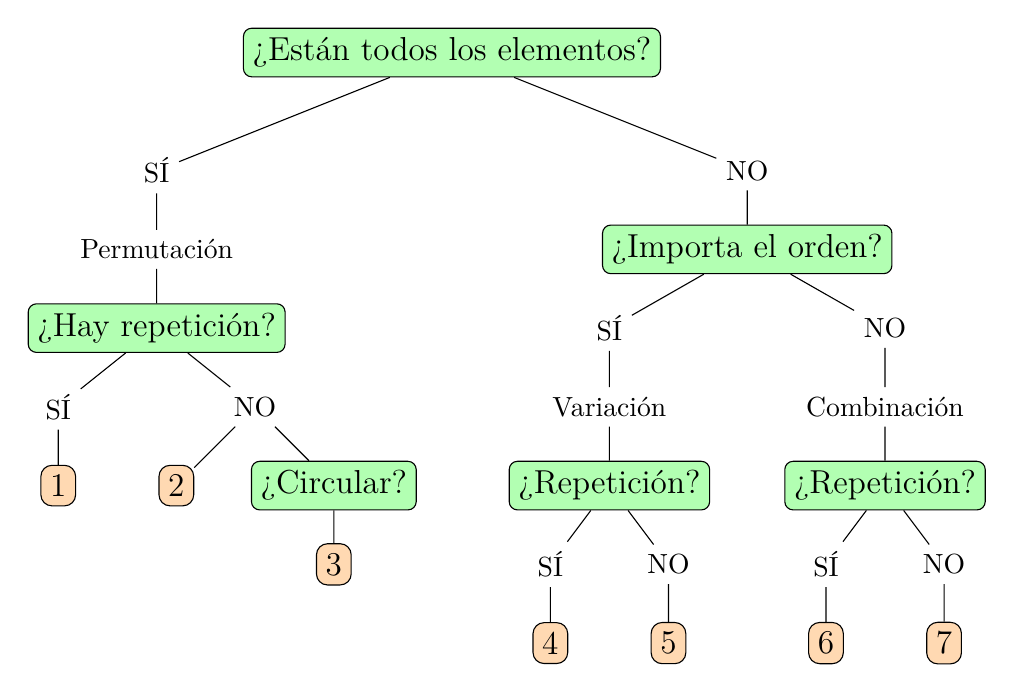
\begin{tikzpicture}[        level 1/.style={sibling distance=7.5cm, level distance=1.5cm},      level 2/.style={sibling distance=2cm, level distance=1cm},      level 3/.style={sibling distance=3.5cm, level distance=1cm},        level 4/.style={sibling distance=2.5cm, level distance=1cm},        level 5/.style={sibling distance=2cm, level distance=1cm},      level 6/.style={sibling distance=1.5cm, level distance=1cm},        arestas/.style={rectangle,rounded corners=4pt,fill=orange!30,draw=black,font=\large},       berdex/.style={rectangle,rounded corners=3pt,fill=green!30,draw=black,font=\large}  ]
    \node[berdex]{¿Están todos los elementos?}
    child{
        node{SÍ}
        child{
            node{Permutación}
            child{
                node[berdex]{¿Hay repetición?}
                child{
                    node{SÍ}
                    child{
                        node[arestas]{1}
                    }
                }
                child{
                    node{NO}
                    child{
                        node[arestas]{2}
                    }
                        child{
                        node[berdex]{¿Circular?}
                            child{
                            node[arestas]{3}
                            }
                    }   
                }
            }
        }
    }
    child{
        node{NO}
        child{
            node[berdex]{¿Importa el orden?}
            child{
                node{SÍ}
                child{
                    node{Variación}
                    child{
                        node[berdex]{¿Repetición?}
                        child{
                            node{SÍ}
                            child{
                                node[arestas]{4}
                            }
                        }
                        child{
                            node{NO}
                            child{
                                node[arestas]{5}
                            }
                        }
                    }
                }
            }
            child{
                node{NO}
                child{
                    node{Combinación}
                    child{
                        node[berdex]{¿Repetición?}
                        child{
                            node{SÍ}
                            child{
                                node[arestas]{6}
                            }
                        }
                        child{
                            node{NO}
                            child{
                                node[arestas]{7}
                            }
                        }
                    }
                }
            }
        }    
    };
    \end{tikzpicture}   
\end{center}

\hfill\break

\begin{itemize}
\tightlist
\item
  ¿Están todos los elementos? No.~La población (15) no es igual a la
  muestra (4).
\item
  ¿Importa el orden? Sí. Se obtienen mejores beneficios siendo el primer
  elegido.
\item
  ¿Hay repetición? Sí. Un mismo estudiante puede ser selccionado más de
  una vez.
\item
  Entonces, estamos ante un caso de Variación Con Repetición (Opción 4):
\end{itemize}

\hfill\break

\includegraphics[width=11.5cm,height=\textheight]{vcr01_01b.png}

\hfill\break

Sabiendo que \(n=15\) (población) y que \(k=4\) (muestra), reemplazamos
en la fórmula:

\includegraphics[width=4.5cm,height=\textheight]{vcr01_01c.png}

\hfill\break

Por tanto, puedo escoger a los 4 estudiantes de 50625 maneras
diferentes.

\hypertarget{meta-information}{%
\section{Meta-information}\label{meta-information}}

exname: VariacionConRep\_01\_py(single-choice) extype: schoice
exsolution: 1000 exshuffle: TRUE

\end{document}
